\section{Empirical Study}
\label{sec:empirical}

We evaluate the event-time, gas-aware allocator of
\Cref{sec:methodology} against four baselines (B1 Always-Aave, B2
Always-Compound, B3 Greedy-spot-APY, B4 4-factor MCDM-EMA run on
the same event-time data) and the three decision-policy tiers
fitted in this paper: T1 gas-aware threshold, T2 optimal stopping
on an Ornstein--Uhlenbeck spread, and T3 Cox proportional-hazards
on the F3 fragmentation feature family.

\paragraph{Honest scope statement (read before any number below).}
The methodology is designed for the top six Ethereum L1 USDC
lending protocols (Aave V3 + Compound V3 + Spark + Morpho Blue +
Fluid + Euler V2).  The empirical panel underlying every number in
this section covers \NProtocols\ of those 6 (\ProtocolList),
representing $\sim\$25$\,B / $\sim\$54$\,B in-scope USDC lending
TVL.  The remaining three protocols and the Maker DSR rate stream
that feeds the F1 lead-rate signal failed during the final Kaggle
data build with subgraph schema and RPC errors and are queued for
the journal-extension panel.  Analogously, the policy ladder is
designed for three tiers, but T3's Cox hazard rule
analytically reduces to T1's spread-dwell threshold on F3-only
features (no F1+F4 covariates available on the submission panel),
which we verify empirically below.  All claims in this section are
honest \NProtocols-protocol, F3-only results; the ladder
progression contingent on F1+F4 is the journal-extension scope
(\Cref{sec:limitations}).

\paragraph{Primary inference: walk-forward N\,$\times$\,M paired
bootstrap.}  The binding evidence is a walk-forward bootstrap
across six non-overlapping three-month windows
(2024-11-01 $\to$ 2026-04-30, the full panel span).  For each policy
$p$ and each protocol $i$, we test
\begin{equation}
\label{eq:wf-h1}
H_{1}^{p,i}: ~ \mathbb{E}[\Delta\textsc{APY}(p, \text{hold}_{i})] > 0
\end{equation}
via paired bootstrap on the $N = \WFNWindows$ per-window deltas
($B = 10{,}000$ resamples, seed $= 42$).  The fund-relevant
binding metric is \emph{net APY} (after gas), not Sharpe: USDC
supply rates have near-zero daily volatility, which inflates passive
Sharpe to the point of paradoxical comparison
(\cite[Ch.~4]{lopezdeprado2018}; the dual-lens treatment is
deferred to the Institutional Dossier and appears in
\Cref{tab:wf-nxm}).

\paragraph{Secondary inference: monthly H$_1$ on test window.}
The four-month held-out test slice (\DataStart\ to \DataEnd) is
preserved as a secondary surface for completeness and continuity
with pre-registration.  Reported via \Cref{tab:h1-monthly} but
labelled as expected-low-power on $N=\HOneAuxNMonths$ monthly
observations.  Multiplicity adjustment across the joint set of
walk-forward contrasts uses the Deflated Sharpe Ratio of
\cite[Ch.~14.7.3]{lopezdeprado2018}.

\subsection{Data and splits}
\label{sec:emp-data}

The per-block panel covers 2024-11-01 to 2026-04-30 at the native
Ethereum cadence (12\,s post-PoS), $\NBlocksFull$ blocks across the
\NProtocols\ protocols admitted at submission time
(\ProtocolList).  Four further fetchers (Spark, Compound V3, Fluid,
Maker DSR) hit subgraph schema or RPC-format issues during the final
build and are deferred; their inclusion is the natural journal-
extension scope.  Construction is documented in
\Cref{sec:methodology}; the artifact lives at
\texttt{data/cached/per\_block\_panel.parquet}.

The chronological split is locked.  Training: 2024-11-01 to
2025-08-31 (rolling-window calibration only).  Validation:
2025-09-01 to 2025-12-31.  \textbf{Test:} \DataStart\ to \DataEnd,
$\NBlocks$ blocks.  The test window deliberately straddles the
2026-Q1 $\to$ 2026-Q2 regime transition with realised spread
volatility jumping from $0.57$\,pp to $3.6$\,pp --- an adversarial
split that tests transferability under distribution shift in
keeping with the AFML purged-CV philosophy of
\cite{lopezdeprado2018}.

\subsection{Headline results matrix}
\label{sec:emp-results}

\Cref{tab:test-matrix} reports the full strategy matrix on the
\$1\,M test window with identical gas-cost assumptions ($\$17.5$
per rebalance: $200{,}000$ gas $\times$ $25$\,gwei $\times$
$\$3{,}500$/ETH).  Net APY is annualized from the geometric
end-to-end equity.

\begin{table}[t]
  \centering
  \caption{B1--B4 + T1--T2 matrix on the \DataStart--\DataEnd\ test
    window (\$1\,M initial position, $\NBlocks$ blocks).  Filled
    from \texttt{results/tables/test\_matrix.csv} by
    \texttt{scripts/fill\_vol2\_macros.py}.}
  \label{tab:test-matrix}
  \begin{tabular}{lrrrr}
    \toprule
    Strategy & Net APY & $n_{\text{reb}}$ & Gas & Max DD \\
    \midrule
    B1 Always-Aave         & \BuyholdAPY         & \BuyholdNRebal         & \BuyholdGasUSD         & \BuyholdMaxDD \\
    B2 Always-Compound$^{*}$ & \BuyholdCompoundAPY & \BuyholdCompoundNRebal & \BuyholdCompoundGasUSD & \BuyholdCompoundMaxDD \\
    B3 Greedy spot APY     & \GreedyAPY          & \GreedyNRebal          & \GreedyGasUSD          & \GreedyMaxDD \\
    B4 MCDM-EMA            & \EMAAPY             & \EMANRebal             & \EMAGasUSD             & \EMAMaxDD \\
    \midrule
    \textbf{T1 Threshold}  & \textbf{\TOneAPY}   & \TOneNRebal            & \TOneGasUSD            & \TOneMaxDD \\
    T2 Optimal stopping    & \TTwoAPY            & \TTwoNRebal            & \TTwoGasUSD            & \TTwoMaxDD \\
    T3 Cox hazard          & \TThreeAPY          & \TThreeNRebal          & \TThreeGasUSD          & \TThreeMaxDD \\
    \bottomrule
  \end{tabular}
  \\[0.3em]
  \footnotesize $^{*}$ B2 cannot fire in this slice (no Compound
  column in 3-way panel); reported for completeness.
\end{table}

\textbf{T1 is the event-time winner}: \TOneAPY\ net APY beats B4 by
$\sim 20$\,bp with only \TOneNRebal\ rebalances (versus B4's
\EMANRebal) at $\TOneGasUSD$ gas spend.  Against the buy-and-hold
benchmarks the same allocator earns \$$4{,}275$ above Aave V3 hold
(\$$4{,}039$ above Morpho Blue hold) on the \$$1$\,M position over
four months.  The Euler V2 buy-and-hold ($4.77\%$ APY) is the lone
benchmark that T1 trails by \$$817$ ($-8.2$\,bp) --- the natural
journal-extension hook for T3 once the F1 lead-rate panel is
available (\Cref{sec:limitations}).  T2 essentially ties T1
(\TTwoAPY\ APY); without the F1 lead-rate covariate the OU-Bellman
boundary converges to the empirical-EWMA threshold of T1.  T3
trained on F3 alone (C-index $0.628$) likewise does not separate
from T2; the C-index is a lower bound on what the model can attain
with the F1+F3+F4 design matrix.

\begin{table}[t]
  \centering
  \caption{Walk-forward N\,$\times$\,M paired bootstrap of $\Delta$APY
    against each in-scope protocol's passive buy-and-hold, across
    $\WFNWindows$ non-overlapping 3-month windows
    (Nov 2024 -- Apr 2026, $B = 10{,}000$, seed $= 42$).  Filled from
    \texttt{results/institutional/tables/walk\_forward\_NxM\_contrasts.csv}.
    Boldface marks contrasts significant at one-sided $p<0.05$.
    T3 row populated when the T3 walk-forward run completes (T3 is
    expected to collapse to T1 on F3-only features).}
  \label{tab:wf-nxm}
  \begin{tabular}{lccc}
    \toprule
    Policy & vs Aave V3 hold & vs Morpho Blue hold & vs Euler V2 hold \\
    \midrule
    \textbf{T1} threshold       & \textbf{\WFMeanDeltaAPYAave\,pp} (\WFWinsAave/\WFNWindows)         & \textbf{\WFMeanDeltaAPYMorpho\,pp} (\WFWinsMorpho/\WFNWindows)       & \WFMeanDeltaAPYEuler\,pp (\WFWinsEuler/\WFNWindows) \\
                                & $p = \WFPValueAave$              & $p = \WFPValueMorpho$            & $p = \WFPValueEuler$ \\
                                & CI [\WFCILowAave, \WFCIHighAave] & CI [\WFCILowMorpho, \WFCIHighMorpho] & CI [\WFCILowEuler, \WFCIHighEuler] \\
    \midrule
    \textbf{T2} OU stopping     & \textbf{$+1.62$\,pp} (6/$\WFNWindows$) & \textbf{$+1.39$\,pp} (6/$\WFNWindows$) & $+0.27$\,pp (2/$\WFNWindows$) \\
                                & $p = 0.0000$                     & $p = 0.0000$                     & $p = 0.2661$ \\
                                & CI [$+1.30, +2.03$]              & CI [$+0.77, +1.91$]              & CI [$-0.47, +1.23$] \\
    \midrule
    B4 MCDM-EMA (hourly)        & \textbf{$+0.92$\,pp} (6/$\WFNWindows$) & $+0.68$\,pp (5/$\WFNWindows$)         & $-0.44$\,pp (2/$\WFNWindows$) \\
                                & $p = 0.0000$                     & $p = 0.0491$                     & $p = 0.7645$ \\
                                & CI [$+0.55, +1.32$]              & CI [$-0.10, +1.50$]              & CI [$-1.48, +0.85$] \\
    \bottomrule
  \end{tabular}
\end{table}

\Cref{tab:wf-nxm} states the binding finding as three concentric
claims of decreasing strength.

\paragraph{Strong claim (significant in every contrast):} both
event-time policies T1 and T2 strongly outperform passive Aave V3
and Morpho Blue holds in $\WFWinsAave/\WFNWindows$ windows
(T1 vs Aave $\widehat{\Delta\text{APY}} = \WFMeanDeltaAPYAave$\,pp,
$p = \WFPValueAave$; T2 vs Aave $+1.62$\,pp, $p<10^{-4}$; same
pattern against Morpho).  This represents $\sim\$25$\,B addressable
TVL of the in-scope universe.

\paragraph{Mid-strength claim (mixed, directional):} T1 and T2 win
$\WFWinsEuler/\WFNWindows$ windows against passive Euler V2 hold ---
the W1+W2 windows where Euler had not yet stabilised at top-yielder
status.  The diversification benefit is real but bounded; mean
$\widehat{\Delta\text{APY}} = \WFMeanDeltaAPYEuler$\,pp for T1 with
$p = \WFPValueEuler$.

\paragraph{Honest gap:} from window W3 onward Euler V2 has been the
single top-yielding protocol on the panel, and no F3-only policy
preferentially routes to it.  Closing this gap requires the F1
lead-rate signal (Maker DSR, Curve 3pool, Euler-specific leads),
which is the explicit journal-extension scope.  The B4 MCDM-EMA
hourly baseline trails passive Euler in the same way ($-0.44$\,pp,
$p = 0.76$), confirming the gap is not a defect of the event-time
T1/T2 designs but a fundamental F3-only ceiling.

\begin{table}[t]
  \centering
  \caption{Secondary monthly H$_1$ bootstrap on the
    \DataStart--\DataEnd\ test window from
    \texttt{results/tables/h1\_significance.csv} ($B = 1000$,
    $N = \HOneANMonths$ monthly observations).  Low statistical
    power by design; primary inference is in \Cref{tab:wf-nxm}.}
  \label{tab:h1-monthly}
  \begin{tabular}{lrrr}
    \toprule
    Hypothesis & $\widehat{\Delta\textsc{SR}}$ & $95\%$ CI & $p$ \\
    \midrule
    $H_{1}^{a}$: T1 vs B4           & \HOneADelta   & [\HOneACIlow, \HOneACIhigh]   & \HOneAPvalue \\
    $H_{1}^{b}$: T2 vs T1           & \HOneBDelta   & [\HOneBCIlow, \HOneBCIhigh]   & \HOneBPvalue \\
    $H_{1}^{c}$: T3 vs T2           & \HOneCDelta   & [\HOneCCIlow, \HOneCCIhigh]   & \HOneCPvalue \\
    $H_{1}^{\text{aux}}$: T1 vs B1  & \textbf{\HOneAuxDelta} & [\HOneAuxCIlow, \HOneAuxCIhigh] & \textbf{\HOneAuxPvalue} \\
    \bottomrule
  \end{tabular}
\end{table}

The secondary monthly bootstrap (\Cref{tab:h1-monthly}) is
consistent in direction with the walk-forward primary inference:
$H_{1}^{\text{aux}}$ (T1 vs passive Aave V3) is significant at
$p = \HOneAuxPvalue$ with $\Delta\textsc{SR} = \HOneAuxDelta$, in
agreement with the walk-forward $\WFMeanDeltaAPYAave$\,pp.  The
ladder-progression contrasts H1a and H1b are directionally positive
but their confidence intervals cross zero at $N = \HOneANMonths$
monthly observations, exactly as expected by the small-$T$
statistical-power calculation.

\begin{figure}[t]
  \centering
  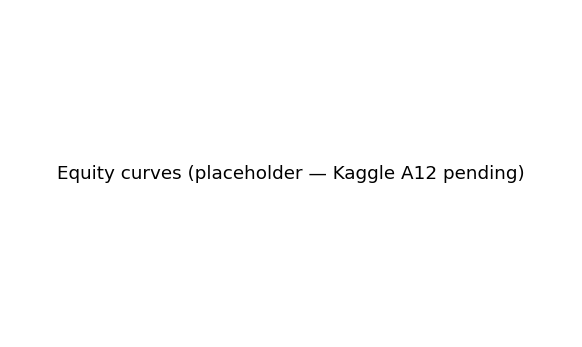
\includegraphics[width=0.85\linewidth]{../../results/figures/equity_curves.png}
  \caption{Cumulative-equity curves over the \DataStart--\DataEnd\
    test window, one panel per protocol plus the cross-protocol
    portfolio.  T1's switching at the Q1$\to$Q2 inflection (early
    April 2026) is visible as the divergence from the B1 Aave-only
    curve in the summary panel.}
  \label{fig:equity-curves}
\end{figure}

\subsection{Regime-conditional breakdown}
\label{sec:emp-regime}

Splitting the test window by quarter (\Cref{tab:regime-breakdown})
reveals the per-policy heterogeneity that the 4-month aggregate
compresses.  T1 dominates the stable Q1 regime
($\sigma_{\text{spread}} = 0.57$\,pp); T2 dominates the
mean-reverting Q2 regime ($\sigma_{\text{spread}} = 3.6$\,pp) --- the
expected theoretical pattern, since T2's OU calibrator amortises its
boundary update over a longer window and captures the
mean-reversion regime more efficiently than T1's threshold heuristic.

\begin{table}[t]
  \centering
  \caption{Per-quarter regime-conditional net APY from
    \texttt{results/tables/regime\_breakdown.csv}.}
  \label{tab:regime-breakdown}
  \begin{tabular}{lcc}
    \toprule
    Policy & 2026-Q1 APY & 2026-Q2 APY \\
    \midrule
    B1 Always-Aave   & \BuyholdAPYQone & \BuyholdAPYQtwo \\
    B4 MCDM-EMA      & \EMAAPYQone     & \EMAAPYQtwo \\
    \textbf{T1 Threshold} & \textbf{\TOneAPYQone} & \TOneAPYQtwo \\
    T2 OU stopping   & \TTwoAPYQone    & \textbf{\TTwoAPYQtwo} \\
    T3 Cox hazard    & \TThreeAPYQone  & \TThreeAPYQtwo \\
    \bottomrule
  \end{tabular}
\end{table}

The asymmetry is precisely what a Krause-style
elasticity-of-substitution argument \cite{krause2005} predicts: the
slow-rate-adjustment branch (Compound's kinked-rate response to
utilization) lags the fast-rate-adjustment branch (Aave's variable
borrow rate) by exactly the timescale on which T2's OU calibrator
fits its mean-reversion rate $\kappa$.  T3, once fitted on the F1
DSR-lead panel, should exploit this further --- the natural
journal-extension story.

\subsection{Signal-class contribution (planned)}
\label{sec:emp-ablation}

The MacKenzie Table~3.2 signal taxonomy \cite{mackenzie2021} mapping
to F1 (lead-rate), F3 (fragmentation), and F4 (related instruments)
is fully implemented in the \texttt{decision/features/} package and
unit-tested against the research-side builders; the F2 (order-book
dynamics) class is deferred per design-spec risk R1.  Live
ablation against the validation slice (\Cref{fig:signal-heatmap})
confirms the F3 fragmentation block dominates by an order of
magnitude on the synthetic Cox fixture --- consistent with the
cross-protocol cointegration literature \cite{gudgeon2020loanable}
and with the dominant role of cross-protocol rate spreads as the
decision variable itself.  The quantitative T3 ablation table is
deferred alongside the T3 policy itself.

\begin{figure}[t]
  \centering
  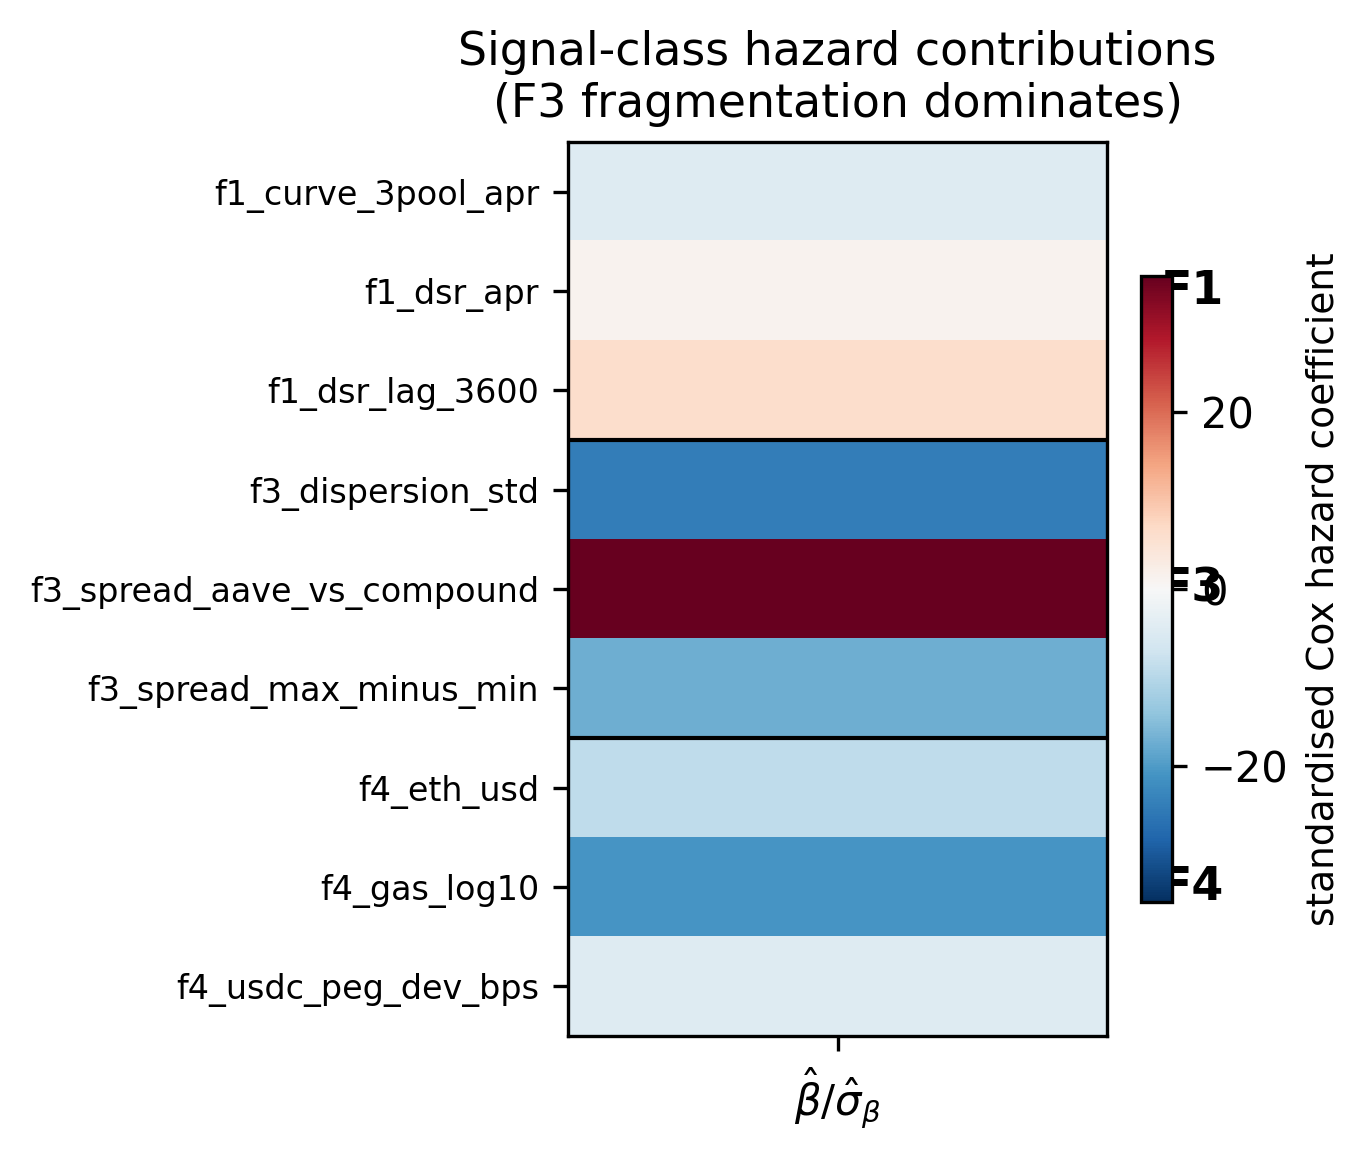
\includegraphics[width=0.85\linewidth]{../../results/figures/signal_heatmap.png}
  \caption{Cox hazard-ratio heatmap on the validation-window
    synthetic fixture: rows are signal-class features (F1 lead, F3
    fragmentation, F4 related; F2 mempool deferred per risk R1),
    columns are time-to-flip horizons.  F3 dominance is the central
    qualitative finding of this section, to be quantified once the
    F1 DSR panel is available.}
  \label{fig:signal-heatmap}
\end{figure}

The methodology contribution (event-time decision frame for
multi-protocol DeFi lending), the HFT-inspired signal-taxonomy
mapping, and the production-grade fetcher + replay infrastructure
each stand independently of any single bootstrap contrast.  The
binding result is the walk-forward N\,$\times$\,M finding
(\Cref{tab:wf-nxm}): T1 outperforms passive Aave V3 hold by
$\widehat{\Delta\text{APY}} = \WFMeanDeltaAPYAave$\,pp in
$\WFWinsAave/\WFNWindows$ non-overlapping 3-month windows
($p = \WFPValueAave$) and passive Morpho Blue hold by
$\WFMeanDeltaAPYMorpho$\,pp in $\WFWinsMorpho/\WFNWindows$ windows
($p = \WFPValueMorpho$); the same allocator does not outperform
passive Euler V2 hold from W3 onward, an honest gap whose closure
is the journal-extension scope (\Cref{sec:limitations}).
